% Provenance (never printed): see sources/outline_sources.md (Year 2: interstellar
% medium, molecular clouds, gravitational collapse and the Jeans criterion, protostars
% and protostellar discs). Curves from figdata/bachelor-2/jeans.py; exercise and problem
% values in the Book 4 scratch calculator calc/ch01.py.
\chapter{Het interstellaire medium en de vorming van sterren}\label{ch:b2:ism-star-formation}

In het sterrenbeeld Stier, op ongeveer \qty{140}{\parsec} van de Zon, wist een donkere
vlek de sterren erachter uit. Met een radiotelescoop afgestemd op de
lijnen van koolstofmonoxide blijkt de vlek een wolk koud gas, zo'n twintigduizend
keer zo zwaar als de Zon en doorweven met filamenten; in de dichtste
knopen worden jonge sterren geboren, en rond een ervan, HL Tauri, vertoont een schijf
van stof een patroon van heldere en donkere ringen waarin zich misschien al planeten
vormen. De Zon, de aarde en elk atoom in de gesteenten van dit boek lagen ooit
in zo'n wolk. Dit hoofdstuk volgt de materie van een planetenstelsel van
het ijle gas tussen de sterren tot een schijf rond een pasgeboren ster: waaruit het
\omterm{def:b2:ism-star-formation:ism}{interstellaire medium} bestaat, waarom een wolk die door haar eigen warmte wordt gedragen
toch ineenstort, hoe lang de ineenstorting duurt, hoe een ster haar massa verzamelt en
waarom de materie die er niet in valt, in een schijf eindigt.

\begin{recall}
Een ster op de hoofdreeks straalt door waterstof tot helium te fuseren in haar
kern en houdt zich met haar druk overeind tegen haar eigen gewicht; haar
plaats in het Hertzsprung--Russell-diagram wordt bepaald door haar massa (natuurkunde,
derde jaar universiteit). Een lichaam op een gesloten baan om een massa $M$ volgt de derde
wet van Kepler, $T^2 = 4\pi^2 a^3/(GM)$ (natuurkunde, eerste jaar universiteit). Een zwart lichaam
met temperatuur $T$ zendt per oppervlakte-eenheid $\sigma T^4$ uit (natuurkunde, tweede jaar
universiteit). In een ideaal gas van $N$ deeltjes is de gemiddelde kinetische energie van
translatie $\tfrac32 N k_{\mathrm B} T$. De parsec,
\qty{3.086e16}{m}, is de afstandseenheid van Boek~3.
\end{recall}

\section{De materie tussen de sterren}

De ruimte tussen de sterren is niet leeg. Nabij de Zon bevat ze gemiddeld ongeveer
één waterstofatoom per kubieke centimeter, een massadichtheid van
\qty{2.7e-24}{g.cm^{-3}}; de lucht die we inademen bevat in hetzelfde volume zo'n $10^{19}$ keer meer
moleculen (\cref{exo:b2:ism-star-formation:1}). Over het Melkwegstelsel verspreid maakt deze ijle
materie toch nog \qtyrange{10}{15}{\percent} uit van de massa van de
galactische schijf.
% ledger: ferriere:mean-density, ferriere:disc-fraction

\begin{definition}[Interstellair medium, interstellair stof]
\label{def:b2:ism-star-formation:ism}
Het \emph{interstellaire medium}\index{interstellair medium} is het gas en stof
dat de ruimte tussen de sterren van een sterrenstelsel vult. Het \emph{interstellaire
stof}\index{interstellair stof} is het deel ervan dat in vaste korrels zit, van enkele
nanometers tot ongeveer een micrometer groot, bestaande uit silicaten, koolstofverbindingen
en, in koude gebieden, ijs.
\end{definition}

Zijn samenstelling is die welke in de Zon en in meteorieten wordt gemeten: in massa
\qty{70.4}{\percent} waterstof, \qty{28.1}{\percent} helium en
\qty{1.5}{\percent} zwaardere elementen. Slechts \qtyrange{0.5}{1}{\percent} van de
massa zit in het stof, en toch bevat het stof het grootste deel van sommige elementen: het gas is
10 tot 100 keer armer dan de Zon aan magnesium, silicium en ijzer, omdat
die atomen in de korrels zijn vastgelegd, terwijl koolstof, stikstof en zuurstof
slechts met factoren 1.2 tot 3 zijn verarmd. De korrels zijn de eerste vaste stoffen van een
toekomstig planetenstelsel; \cref{ch:b2:planet-formation-meteorites}
volgt ze verder.
% ledger: ferriere:composition, ferriere:dust-fraction, ferriere:refractory-depletion

\subsection{Vijf fasen}

Het gas is verre van homogeen. Het komt voor in enkele afzonderlijke toestanden, of fasen,
elk met een eigen bereik van temperatuur en dichtheid (tabel hieronder). Ongeveer de helft
van zijn massa zit in wolken die slechts \qtyrange{1}{2}{\percent} van het volume vullen;
de rest, warm of heet, vult de ruimte daartussen.
% ledger: ferriere:disc-fraction

\begin{table}[htbp]
\centering
\small
\begin{tabular}{lll}
\hline
fase & temperatuur (K) & dichtheid $n$ (\unit{cm^{-3}}) \\
\hline
moleculair & 10--20 & $10^2$--$10^6$ \\
koud atomair & 50--100 & 20--50 \\
warm atomair & 6000--10\,000 & 0.2--0.5 \\
warm geïoniseerd & ongeveer 8000 & 0.2--0.5 \\
heet geïoniseerd & ongeveer $10^6$ & ongeveer 0.0065 \\
\hline
\end{tabular}
\caption{De fasen van het interstellaire gas nabij de Zon; $n$ is de
aantalsdichtheid van waterstofkernen.}
\label{tab:b2:ism-star-formation:phases}
% ledger: ferriere:molecular, ferriere:cold-atomic, ferriere:warm-atomic, ferriere:warm-ionized, ferriere:hot-ionized
\end{table}

De tabel verbergt een regelmaat. De druk van een ideaal gas is
$P = n k_{\mathrm B} T$, dus het product $nT$ is er een maat voor. Voor het koude atomaire
gas is $nT$ ongeveer $30\times75 \approx 2000$ (in \unit{K.cm^{-3}}), voor het warme
atomaire gas ongeveer $0.3\times8000 \approx 2400$, voor het hete gas ongeveer
$0.0065\times10^6 = 6500$: op een factor van enkele na hebben de drie fasen die
de ruimte tussen de wolken delen dezelfde druk (figuur hieronder).
Waar een heet en een koud gas elkaar bij gelijke druk raken, duwt geen van beide het andere
weg; een gas dat bij constante druk afkoelt, wordt evenredig dichter en
valt van de warme fase in de koude. De \omterm{def:b2:ism-star-formation:molecular-cloud}{moleculaire wolken} bereiken veel hogere drukken, tot duizenden keren meer in hun dichte delen: ze worden bijeengehouden door hun eigen zwaartekracht, niet door de
druk van hun omgeving.

\begin{omfigure}
\begin{tikzpicture}
\begin{axis}[omrecord, width=0.86\linewidth, height=6.4cm, xmode=log, ymode=log,
  xmin=1e-3, xmax=1e7, ymin=3, ymax=3e6,
  xlabel={dichtheid van waterstofkernen $n$ (\unit{cm^{-3}})}, ylabel={temperatuur $T$ (K)},
  tick label style={font=\scriptsize}, label style={font=\small}, clip=false,
  legend pos=north east, legend style={font=\scriptsize, draw=black!30}]
\addplot[black!45, densely dashed, domain=1e-3:1e3, samples=2] {3000/x};
\addlegendentry{$nT = \num{3000}$}
\addplot[black!60, densely dotted, thick, domain=0.1:1e5, samples=2] {3e5/x};
\addlegendentry{$nT = 3\times10^5$}
\fill[blue!45, opacity=0.6] (axis cs:1e2,10) rectangle (axis cs:1e6,20);
\fill[teal!50, opacity=0.6] (axis cs:20,50) rectangle (axis cs:50,100);
\fill[orange!55, opacity=0.6] (axis cs:0.2,6000) rectangle (axis cs:0.5,10000);
\fill[red!45, opacity=0.6] (axis cs:0.2,5714) rectangle (axis cs:0.5,11200);
\fill[violet!50, opacity=0.6] (axis cs:0.00464,7.14e5) rectangle (axis cs:0.0091,1.4e6);
\node[font=\scriptsize, anchor=south east] at (axis cs:1e6,20) {moleculaire wolken};
\node[font=\scriptsize, anchor=south west] at (axis cs:50,100) {koud atomair};
\node[font=\scriptsize, anchor=east, align=right] at (axis cs:0.17,8000) {warm atomair\\en warm geïoniseerd};
\node[font=\scriptsize, anchor=west] at (axis cs:0.011,1e6) {heet geïoniseerd};
\end{axis}
\end{tikzpicture}

\par\smallskip{\small De fasen van het interstellaire gas nabij de Zon (bereiken uit de tabel
hierboven; de warme geïoniseerde en de hete fase, als enkele waarden gegeven, zijn getekend als vakjes
van een factor 1.4 breed). Langs elke grijze lijn is de druk $nk_{\mathrm B}T$ constant: de
koude, warme en hete fase liggen dicht bij dezelfde druk, op een factor van enkele na,
terwijl de \omterm{def:b2:ism-star-formation:molecular-cloud}{moleculaire wolken}, gebonden door hun eigen zwaartekracht, drukken tot duizenden keren hoger bereiken.
Gegevens: Ferrière (2001).}
\end{omfigure}

Stof verraadt zich op drie manieren. Het verzwakt het licht van de sterren erachter,
en blauw licht meer dan rood, zodat sterren die erdoor worden gezien roder lijken
dan ze zijn. Het straalt in het verre infrarood en op millimetergolflengten,
bij de temperatuur van enkele tientallen kelvin waartoe het sterlicht het opwarmt. En
het verbergt alles wat binnen een dichte wolk ligt voor optische telescopen; daarom
wordt stervorming waargenomen op radio- en infraroodgolflengten. Het gas wordt
opgespoord via zijn lijnen: atomaire waterstof via zijn radiolijn bij \qty{21}{cm},
moleculaire waterstof, die koud nauwelijks straalt, via de lijnen van de
moleculen die ermee meekomen, met koolstofmonoxide voorop.

\section{Moleculaire wolken}

De koudste en dichtste fase is die waarin sterren ontstaan.

\begin{definition}[Moleculaire wolk, dichte kern]
\label{def:b2:ism-star-formation:molecular-cloud}
Een \emph{moleculaire wolk}\index{moleculaire wolk} is een gebied van het
\omterm{def:b2:ism-star-formation:ism}{interstellaire medium} dat dicht en ondoorzichtig genoeg is om zijn waterstof grotendeels in
moleculen, \ce{H2}, te laten zitten, door stof afgeschermd van het ultraviolette licht van de sterren
dat ze zou splitsen; de temperatuur is ongeveer \qty{10}{K} tot \qty{20}{K}. Een
\emph{dichte kern}\index{dichte kern} is een compacte verdichting in een
moleculaire wolk, enkele tienden van een parsec groot of kleiner, met dichtheden van
$10^4$ tot $10^5$ deeltjes per kubieke centimeter, waaruit één ster of een
kleine groep sterren ontstaat.
\end{definition}

Wolken zijn hiërarchisch georganiseerd (tabel hieronder). Een donkere wolk als die in de Stier
bevat klonten, en de klonten bevatten kernen, elk niveau dichter, kleiner en
rustiger dan het niveau erboven: in een kern beweegt het gas met hoogstens enkele tienden van
een kilometer per seconde, de geluidssnelheid in gas van \qty{10}{K}. Het in
koolstofmonoxide gekarteerde gebied van de Stier bevat ongeveer \num{2.4e4} zonsmassa's
gas; slechts \qtyrange{0.3}{1.2}{\percent} ervan is omgezet in de
jonge sterren die men er ziet, met een tempo van ongeveer acht sterren per honderdduizend
jaar over de laatste drie miljoen jaar. Stervorming is traag en verkwistend.
% ledger: bt07:clouds, bt07:clumps, bt07:cores, goldsmith:taurus-mass, goldsmith:taurus-sfe, goldsmith:taurus-distance

\begin{table}[htbp]
\centering
\small
\begin{tabular}{lccc}
\hline
 & donkere wolken & klonten & \omterm{def:b2:ism-star-formation:molecular-cloud}{dichte kernen} \\
\hline
massa (zonsmassa's) & $10^3$--$10^4$ & 50--500 & 0.5--5 \\
grootte (pc) & 2--15 & 0.3--3 & 0.03--0.2 \\
gemiddelde dichtheid (\unit{cm^{-3}}) & 50--500 & $10^3$--$10^4$ & $10^4$--$10^5$ \\
gastemperatuur (K) & ongeveer 10 & 10--20 & 8--12 \\
voorbeelden & Stier, Musca & --- & L1544, B68 \\
\hline
\end{tabular}
\caption{De hiërarchie van een donkere \omterm{def:b2:ism-star-formation:molecular-cloud}{moleculaire wolk}. De dichtheden tellen alle
deeltjes. Gegevens: Bergin en Tafalla (2007).}
\label{tab:b2:ism-star-formation:hierarchy}
% ledger: bt07:clouds, bt07:clumps, bt07:cores
\end{table}

Waarom zijn de wolken zo koud? Gas verliest energie door fotonen uit te zenden die
ontsnappen, en moleculen zijn efficiënte stralers: een botsing tilt een
koolstofmonoxidemolecuul naar een hoger rotatieniveau, het molecuul valt terug door
een foton op millimetergolflengte uit te zenden, en het foton verlaat de wolk
en neemt de energie van de botsing mee. Het stof, opgewarmd door het zwakke
sterlicht dat binnendringt, straalt in het verre infrarood. De verwarming, door kosmische
straling en door sterlicht dat door het stof is gefilterd, is zwak; het evenwicht ligt
rond \qty{10}{K}. In zulk gas is de thermische druk klein, en kan de zwaartekracht
winnen.

\begin{omfigure}
\begin{minipage}[c]{0.44\linewidth}
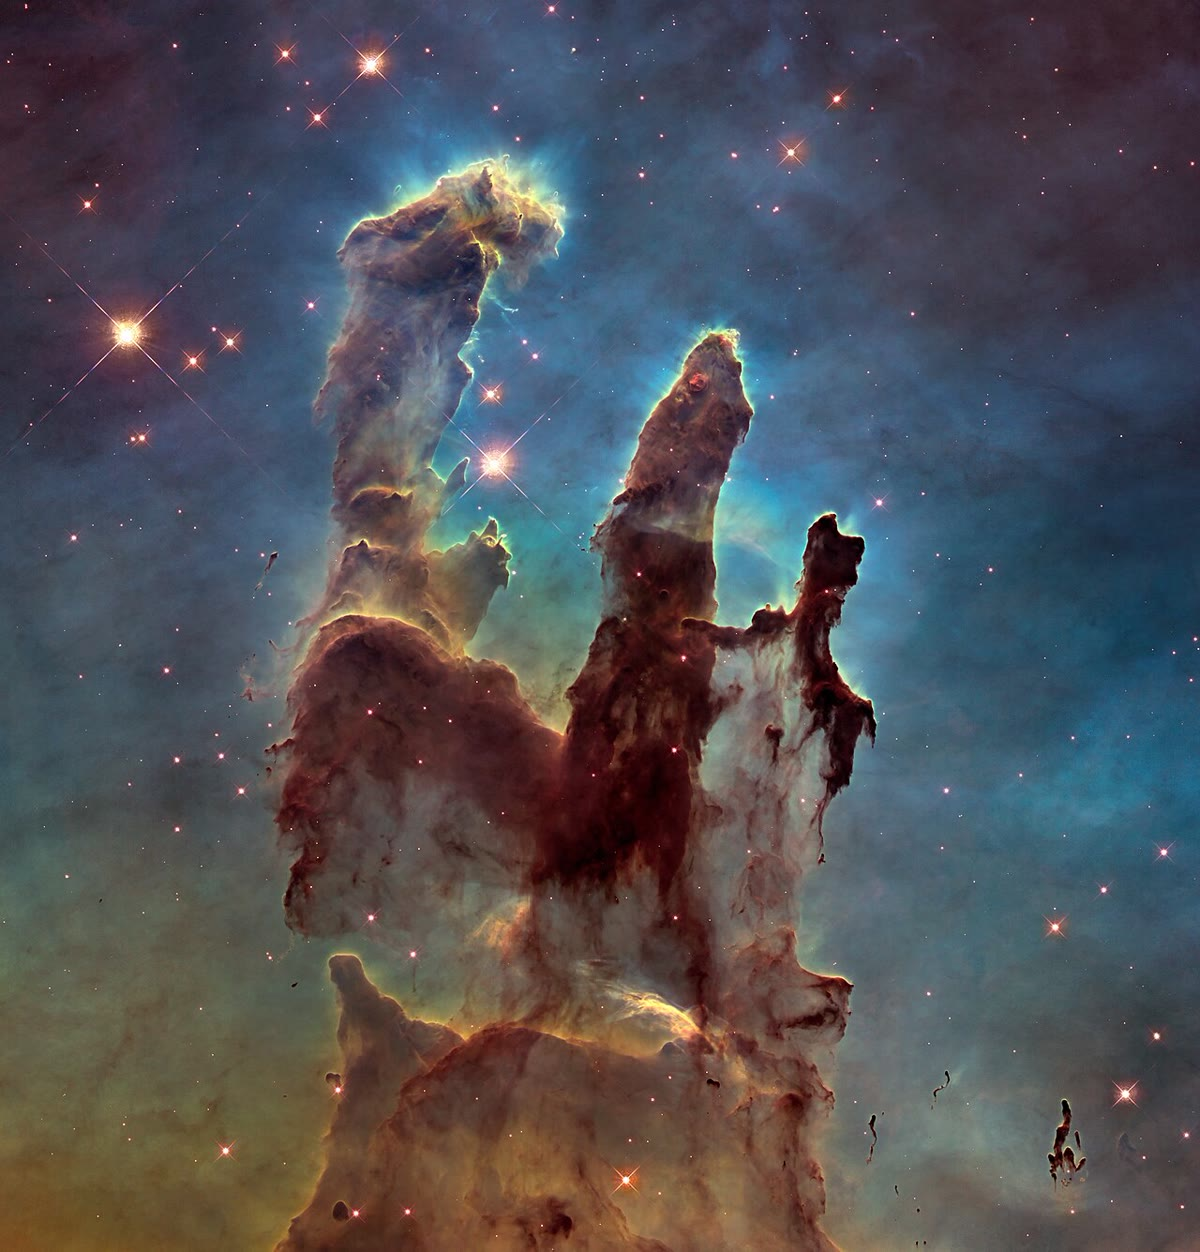
\includegraphics[width=\linewidth]{images/book4/b2-pillars-of-creation.jpg}
\end{minipage}\hfill
\begin{minipage}[c]{0.52\linewidth}
{\small De ``Pilaren van de Schepping'' in de Adelaarnevel, in zichtbaar licht vastgelegd door de
ruimtetelescoop Hubble. De zuilen bestaan uit koud, dicht moleculair gas en
stof, lichtjaren lang, aangevreten en van bovenaf belicht door het ultraviolette licht van
zware jonge sterren buiten beeld; het stof maakt ze ondoorzichtig. Kleine
verdichtingen aan hun toppen vormen sterren. NASA, ESA en het Hubble
Heritage Team (STScI/AURA), publiek domein.}
\end{minipage}
\end{omfigure}

\section{Gravitationele ineenstorting}

Een wolk is een evenwicht tussen twee energieën: de thermische energie van haar gas,
die naar buiten duwt, en haar gravitatie-energie, die naar binnen trekt. De
tweede groeit sneller met de massa dan de eerste; boven een bepaalde massa wint de
zwaartekracht.

\begin{proposition}[Gravitatie-energie van een homogene bol]
\label{prop:b2:ism-star-formation:grav-energy}
Een bol met homogene dichtheid, massa $M$ en straal $R$ heeft de
gravitationele potentiële energie
\[
  U = -\frac{3}{5}\,\frac{G M^2}{R}.
\]
\end{proposition}

\begin{proof}
Bouw de bol schil voor schil op. Wanneer zijn straal $r$ is, heeft hij de massa
$m(r) = M r^3/R^3$; een schil met dikte $\mathrm dr$ en massa
$\mathrm dm = 3M r^2\,\mathrm dr/R^3$ vanuit het oneindige naar zijn oppervlak brengen, maakt
de energie $G m(r)\,\mathrm dm/r$ vrij, omdat een bol daarbuiten aantrekt alsof
zijn massa in zijn middelpunt zat (de schilstelling, natuurkunde). Dus
\[
  U = -\int_0^R \frac{G}{r}\,\frac{M r^3}{R^3}\,\frac{3 M r^2}{R^3}\,\mathrm dr
    = -\frac{3 G M^2}{R^6}\int_0^R r^4\,\mathrm dr = -\frac{3}{5}\,\frac{G M^2}{R}.
  \qedhere
\]
\end{proof}

Een zichzelf aantrekkend lichaam in evenwicht volgt de viriaalstelling: gemiddeld
over de tijd is tweemaal zijn kinetische energie plus zijn gravitatie-energie nul,
$2K + U = 0$ (natuurkunde, derde jaar universiteit, waar ze uit de
bewegingsvergelijkingen wordt afgeleid). Voor een wolk in rust is $K$ de thermische energie van haar
deeltjes. Als $2K > |U|$, zet het gas uit; als $2K < |U|$, heeft de zwaartekracht geen
evenwicht dat haar tegenwerkt, en trekt de wolk samen.

\begin{proposition}[Jeans-criterium]\label{prop:b2:ism-star-formation:jeans}
Een homogene, isotherme wolk met temperatuur $T$ en dichtheid $\rho$, bestaande uit
deeltjes met gemiddelde massa $\mu m_u$, stort onder haar eigen zwaartekracht in als haar massa
groter is dan de \emph{\omterm{def:b2:ism-star-formation:jeans}{Jeans-massa}}
\[
  M_J = \left(\frac{5 k_{\mathrm B} T}{G\mu m_u}\right)^{3/2}
        \left(\frac{3}{4\pi\rho}\right)^{1/2},
\]
of, wat op hetzelfde neerkomt, als haar straal groter is dan de \emph{\omterm{def:b2:ism-star-formation:jeans}{Jeans-lengte}}
\[
  R_J = \left(\frac{15 k_{\mathrm B} T}{4\pi G\mu m_u\,\rho}\right)^{1/2}.
\]
Dit is het \emph{Jeans-criterium}\index{Jeans-criterium}.
\end{proposition}

\begin{proof}
De wolk bevat $N = M/(\mu m_u)$ deeltjes, met de thermische energie
$K = \tfrac32 N k_{\mathrm B}T = \tfrac32 M k_{\mathrm B}T/(\mu m_u)$. Volgens
\cref{prop:b2:ism-star-formation:grav-energy} stort ze in als
$2K < \tfrac35 GM^2/R$, dat wil zeggen
\[
  \frac{3 M k_{\mathrm B} T}{\mu m_u} < \frac{3}{5}\,\frac{G M^2}{R}
  \iff M > \frac{5 k_{\mathrm B} T}{G \mu m_u}\, R .
\]
Elimineer $R$ met $M = \tfrac43\pi R^3\rho$, dat wil zeggen $R = (3M/4\pi\rho)^{1/3}$:
$M^{2/3} > \frac{5 k_{\mathrm B}T}{G\mu m_u}\,(3/4\pi\rho)^{1/3}$, en beide leden
tot de macht $3/2$ verheffen geeft $M > M_J$. Elimineert men in plaats daarvan $M$, dan geeft
$\tfrac43\pi R^3\rho > 5 k_{\mathrm B}T R/(G\mu m_u)$ de ongelijkheid $R^2 > 15
k_{\mathrm B}T/(4\pi G\mu m_u\rho)$, dat wil zeggen $R > R_J$.
\end{proof}

\begin{definition}[Jeans-massa, Jeans-lengte]\label{def:b2:ism-star-formation:jeans}
De \emph{Jeans-massa}\index{Jeans-massa} $M_J$ en de \emph{Jeans-lengte}\index{Jeans-lengte} $R_J$ van een gas met gegeven temperatuur en dichtheid
zijn de massa en de straal waarboven een homogene bol van dat gas
onder zijn eigen zwaartekracht ineenstort
(\cref{prop:b2:ism-star-formation:jeans}).
\end{definition}

De \omterm{def:b2:ism-star-formation:jeans}{Jeans-massa} groeit als $T^{3/2}$ en daalt als $\rho^{-1/2}$: koud, dicht gas
stort het gemakkelijkst in. In een \omterm{def:b2:ism-star-formation:molecular-cloud}{moleculaire wolk} is de gemiddelde massa per deeltje
$\mu = 2.33$ atomaire massa-eenheden: moleculaire waterstof met één heliumatoom op
ongeveer elke vijf moleculen. Bij \qty{10}{K} en $10^4$ deeltjes per kubieke
centimeter is $\rho = \mu m_u n = \qty{3.87e-17}{kg.m^{-3}}$ en
$M_J = 5.5$ zonsmassa's, binnen een \omterm{def:b2:ism-star-formation:jeans}{Jeans-lengte} van \qty{0.13}{\parsec}:
de massa en de grootte van een \omterm{def:b2:ism-star-formation:molecular-cloud}{dichte kern}. Bij de gemiddelde dichtheid van een donkere wolk,
$100$ deeltjes per kubieke centimeter, is de \omterm{def:b2:ism-star-formation:jeans}{Jeans-massa} tien keer groter, 55
zonsmassa's, en een wolk van \num{24000} zonsmassa's zoals die in de Stier bevat er
honderden (figuur hieronder).
% ledger: kauffmann:mu, nist:u, const:kB, const:G, sun:mass, goldsmith:taurus-mass

\begin{omfigure}
\begin{tabular}{@{}c@{\hspace{3mm}}c@{}}
\begin{tikzpicture}
\begin{axis}[omrecord, width=0.455\linewidth, height=6.0cm, xmode=log, ymode=log,
  xmin=10, xmax=1e7, ymin=0.05, ymax=1e4,
  xlabel={$n$ (\unit{cm^{-3}})}, ylabel={Jeans-massa (zonsmassa's)},
  tick label style={font=\scriptsize}, label style={font=\small},
  legend style={font=\scriptsize, at={(0.97,0.97)}, anchor=north east, draw=none, fill=white, fill opacity=0.85}]
\fill[blue!12] (axis cs:1e4,0.5) rectangle (axis cs:1e5,5);
\node[font=\scriptsize, blue!50!black, anchor=north east] at (axis cs:1e5,0.5) {dichte kernen};
\addplot[very thick, blue!70!black] table[x=n, y=MJ10] {figdata/out/bachelor-2-jeans-jeans.dat};
\addlegendentry{\qty{10}{K}}
\addplot[very thick, orange!80!black] table[x=n, y=MJ20] {figdata/out/bachelor-2-jeans-jeans.dat};
\addlegendentry{\qty{20}{K}}
\addplot[very thick, red!75!black] table[x=n, y=MJ50] {figdata/out/bachelor-2-jeans-jeans.dat};
\addlegendentry{\qty{50}{K}}
\end{axis}
\end{tikzpicture}
&
\begin{tikzpicture}
\begin{axis}[omrecord, width=0.455\linewidth, height=6.0cm, xmode=log, ymode=log,
  xmin=10, xmax=1e7, ymin=0.01, ymax=20,
  xlabel={$n$ (\unit{cm^{-3}})}, ylabel={vrijevaltijd (Myr)},
  tick label style={font=\scriptsize}, label style={font=\small}]
\addplot[very thick, black!70] table[x=n, y=tff_Myr] {figdata/out/bachelor-2-jeans-tff.dat};
\fill[blue!12] (axis cs:1e4,0.05) rectangle (axis cs:1e5,0.5);
\addplot[very thick, black!70] table[x=n, y=tff_Myr] {figdata/out/bachelor-2-jeans-tff.dat};
\node[font=\scriptsize, blue!50!black, anchor=north] at (axis cs:3.2e4,0.05) {kernen};
\end{axis}
\end{tikzpicture}
\\[2pt]
{\small (a) \omterm{def:b2:ism-star-formation:jeans}{Jeans-massa}} & {\small (b) \omterm{def:b2:ism-star-formation:free-fall}{vrijevaltijd}}
\end{tabular}

\par\smallskip{\small (a) De \omterm{def:b2:ism-star-formation:jeans}{Jeans-massa} tegen de deeltjesdichtheid voor drie
temperaturen ($\mu = 2.33$). Het gearceerde vak geeft de massa's en dichtheden van
waargenomen \omterm{def:b2:ism-star-formation:molecular-cloud}{dichte kernen}: bij \qty{10}{K} ligt hun massa dicht bij de \omterm{def:b2:ism-star-formation:jeans}{Jeans-massa}. (b) De
\omterm{def:b2:ism-star-formation:free-fall}{vrijevaltijd} van \cref{prop:b2:ism-star-formation:free-fall}: een derde van een miljoen
jaar bij $10^4$ deeltjes per kubieke centimeter, tien keer langer bij $10^2$.}
\end{omfigure}

Een wolk die begint in te storten, wordt dichter, en haar \omterm{def:b2:ism-star-formation:jeans}{Jeans-massa} daalt als
$\rho^{-1/2}$ zolang ze koud blijft, wat ze doet zolang ze de
compressiewarmte kan wegstralen. Delen van de wolk worden dan op zichzelf instabiel
en storten afzonderlijk in: de wolk \emph{fragmenteert}. Daarom ontstaan sterren
in groepen en zijn hun massa's klein vergeleken met de wolken waaruit ze
voortkomen. De fragmentatie stopt wanneer het gas te dicht wordt om zijn straling te laten
ontsnappen: de compressiewarmte wordt vastgehouden, de temperatuur stijgt, en de
\omterm{def:b2:ism-star-formation:jeans}{Jeans-massa} daalt niet verder.

Hoe lang duurt een ineenstorting? Als de druk verwaarloosbaar is, valt elke schil van de
wolk vrij naar het middelpunt.

\begin{proposition}[Vrijevaltijd]\label{prop:b2:ism-star-formation:free-fall}
Een homogene bol met dichtheid $\rho$, aanvankelijk in rust en zonder druk,
stort naar zijn middelpunt in in de tijd
\[
  t_{\mathrm{ff}} = \left(\frac{3\pi}{32\,G\rho}\right)^{1/2},
\]
onafhankelijk van zijn straal.
\end{proposition}

\begin{proof}
Beschouw een deeltje in rust op afstand $R$ van het middelpunt, aan het
oppervlak van de bol. De schillen binnen hem vallen sneller of met hem mee, nooit
achter hem, dus de massa $M = \tfrac43\pi R^3\rho$ die hem aantrekt, blijft de hele weg
dezelfde. Zijn baan is een ontaarde Keplerbaan: een ellips die is platgedrukt tot
een recht lijnstuk, met het verre uiteinde in $R$ en het aantrekkingscentrum aan
het andere uiteinde, zodat de halve lange as $a = R/2$ is. De val van het verre uiteinde
naar het middelpunt duurt een halve periode; volgens de derde wet van Kepler
\[
  t_{\mathrm{ff}} = \frac12\cdot 2\pi\sqrt{\frac{(R/2)^3}{GM}}
  = \pi\sqrt{\frac{R^3}{8\,G\cdot\frac43\pi R^3\rho}}
  = \sqrt{\frac{3\pi}{32\,G\rho}} .
\]
$R$ valt weg: elke schil van een homogene bol komt op hetzelfde
ogenblik in het middelpunt aan.
\end{proof}

\begin{definition}[Vrijevaltijd]\label{def:b2:ism-star-formation:free-fall}
De \emph{vrijevaltijd}\index{vrijevaltijd} van een gas met dichtheid $\rho$ is
$t_{\mathrm{ff}} = (3\pi/32G\rho)^{1/2}$, de tijd die een homogene bol met die
dichtheid nodig zou hebben om alleen onder zijn eigen zwaartekracht in te storten.
\end{definition}

Voor een \omterm{def:b2:ism-star-formation:molecular-cloud}{dichte kern} van $10^4$ deeltjes per kubieke centimeter is de \omterm{def:b2:ism-star-formation:free-fall}{vrijevaltijd}
\qty{0.34}{Myr}; voor een hele donkere wolk van $10^2$ \qty{3.4}{Myr}. Als elke
\omterm{def:b2:ism-star-formation:molecular-cloud}{moleculaire wolk} van het Melkwegstelsel in één \omterm{def:b2:ism-star-formation:free-fall}{vrijevaltijd} ineenstortte en in
sterren overging, zou het Melkwegstelsel veel sneller sterren vormen dan het doet: in de Stier is het gas dat
de laatste drie miljoen jaar werkelijk in sterren is omgezet ongeveer één procent van de wolk. De
wolken worden afgeremd, door turbulente bewegingen en door magneetvelden die de
geïoniseerde fractie van het gas meesleept, en het meeste van hun gas wordt verspreid door
de winden en het licht van de eerste zware sterren voordat het kan ineenstorten: vandaar
het lage rendement dat in de Stier wordt gemeten.
% ledger: bt07:tff

\begin{history}[James Jeans]
James Jeans (1877--1946) publiceerde in 1902 de analyse van de stabiliteit van een
gas onder zijn eigen zwaartekracht waaruit de \omterm{def:b2:ism-star-formation:jeans}{Jeans-massa} en -lengte voortkomen. Hij
bestudeerde de groei van kleine dichtheidsgolven in een oneindig homogeen gas en
vond dat golven die langer zijn dan een kritische lengte niet door de druk worden tegengewerkt,
maar groeien: het gas valt uiteen in verdichtingen van ongeveer die grootte. Zijn kritische
lengte verschilt slechts met een numerieke factor van de hierboven gevonden straal; de
fysica, zwaartekracht tegen thermische druk, is dezelfde.
\end{history}

\section{Protosterren}

De ineenstorting van een kern is niet homogeen. Het iets dichtere centrum valt
eerst; daar vormt zich een klein, dicht, heet object dat groeit door het gas op te slokken
dat erop blijft neerregenen.

\begin{definition}[Protoster]\label{def:b2:ism-star-formation:protostar}
Een \emph{protoster}\index{protoster} is een ster in wording die nog het grootste
deel van haar massa wint door accretie van het gas van haar moederkern; ze
straalt door de energie die het vallende gas vrijmaakt, niet door kernfusie.
\end{definition}

Hoe snel groeit een \omterm{def:b2:ism-star-formation:protostar}{protoster}? Een kern op het punt van ineenstorten bevat ongeveer een \omterm{def:b2:ism-star-formation:jeans}{Jeans-massa}
en valt in ongeveer een \omterm{def:b2:ism-star-formation:free-fall}{vrijevaltijd}, dus de massa komt aan met een tempo in de orde van
$M_J/t_{\mathrm{ff}}$.

\begin{proposition}[Accretietempo van een protoster]
\label{prop:b2:ism-star-formation:accretion}
Zij $c_s = (k_{\mathrm B}T/\mu m_u)^{1/2}$ de isotherme geluidssnelheid
van het gas van een kern. De verhouding van de \omterm{def:b2:ism-star-formation:jeans}{Jeans-massa} tot de \omterm{def:b2:ism-star-formation:free-fall}{vrijevaltijd} hangt
niet af van de dichtheid, en
\[
  \frac{M_J}{t_{\mathrm{ff}}} \approx 10\,\frac{c_s^3}{G}:
\]
een \omterm{def:b2:ism-star-formation:protostar}{protoster} groeit met een tempo in de orde van $c_s^3/G$, dat alleen door de temperatuur van haar
kern wordt bepaald.
\end{proposition}

\begin{proof}
Met $k_{\mathrm B}T/(\mu m_u) = c_s^2$ is $M_J = 5^{3/2}\,c_s^3\,G^{-3/2}
(3/4\pi\rho)^{1/2}$ en $t_{\mathrm{ff}} = (3\pi/32)^{1/2}(G\rho)^{-1/2}$, dus
\[
  \frac{M_J}{t_{\mathrm{ff}}} = 5^{3/2}\left(\frac{3}{4\pi}\right)^{1/2}
  \left(\frac{32}{3\pi}\right)^{1/2}\frac{c_s^3}{G}
  = 11.18\times0.489\times1.84\,\frac{c_s^3}{G} \approx 10\,\frac{c_s^3}{G},
\]
waarin $\rho$ is weggevallen. De factor hangt af van de vorm van de kern;
modellen van kernen waarvan de dichtheid naar buiten afneemt, zoals waargenomen, geven tempo's
dichter bij $c_s^3/G$ zelf.
\end{proof}

Bij \qty{10}{K} is $c_s = \qty{0.19}{km.s^{-1}}$ en is $c_s^3/G$
\num{1.6e-6} zonsmassa per jaar: een ster als de Zon is in ongeveer
\num{600000} jaar opgebouwd, een tijd vergelijkbaar met de \omterm{def:b2:ism-star-formation:free-fall}{vrijevaltijd} van haar kern.
In een warmere kern, bij \qty{20}{K}, is het tempo $2^{3/2} = 2.8$ keer hoger.

\begin{omfigure}
\begin{tikzpicture}[font=\scriptsize]
% panel 1: core
\begin{scope}
\shade[inner color=gray!70, outer color=gray!10] (0,0) circle (1.0);
\node[align=center] at (0,-1.45) {(1) dichte kern\\$\sim\qty{0.1}{pc}$, \qty{10}{K}};
\end{scope}
% panel 2: collapse with infall arrows
\begin{scope}[xshift=3.0cm]
\shade[inner color=gray!80, outer color=gray!10] (0,0) circle (0.9);
\foreach \a in {0,45,...,315} \draw[-{Stealth[length=1.6mm]}, black!70] (\a:0.85) -- (\a:0.3);
\fill[orange!90!red] (0,0) circle (0.07);
\node[align=center] at (0,-1.45) {(2) ineenstorting\\$t_{\mathrm{ff}} \sim \qty{0.1}{Myr}$};
\end{scope}
% panel 3: protostar with disc and outflow
\begin{scope}[xshift=6.0cm]
\fill[gray!25] (0,0) ellipse (0.9 and 0.6);
\fill[brown!55] (0,0) ellipse (0.75 and 0.12);
\fill[orange!90!red] (0,0) circle (0.08);
\fill[blue!25] (0,0.1) -- (-0.22,0.95) -- (0.22,0.95) -- cycle;
\fill[blue!25] (0,-0.1) -- (-0.22,-0.95) -- (0.22,-0.95) -- cycle;
\node[align=center] at (0,-1.45) {(3) protoster, schijf\\en uitstroming, $\sim\qty{0.5}{Myr}$};
\end{scope}
% panel 4: T Tauri with disc
\begin{scope}[xshift=9.0cm]
\fill[brown!55] (0,0) ellipse (0.85 and 0.1);
\fill[yellow!80!orange] (0,0) circle (0.1);
\draw[blue!40, thick] (0,0.15) -- (0,0.6); \draw[blue!40, thick] (0,-0.15) -- (0,-0.6);
\node[align=center] at (0,-1.45) {(4) T-Tauri-ster\\en schijf, 1--\qty{5}{Myr}};
\end{scope}
% panel 5: planetary system
\begin{scope}[xshift=12.0cm]
\fill[yellow!80!orange] (0,0) circle (0.12);
\foreach \r in {0.3,0.5,0.8} \draw[black!40] (0,0) ellipse ({\r} and {0.4*\r});
\fill (0.3,0) circle (0.03); \fill (-0.5,0.03) circle (0.035); \fill (0.8,0.05) circle (0.06);
\node[align=center] at (0,-1.45) {(5) hoofdreeksster\\en planeten};
\end{scope}
\foreach \x in {1.4,4.4,7.4,10.4} \draw[-{Stealth}, thick, black!60] (\x,0) -- (\x+0.25,0);
\end{tikzpicture}

\par\smallskip{\small Van een \omterm{def:b2:ism-star-formation:molecular-cloud}{dichte kern} tot een planetenstelsel (schematisch, niet op schaal).
(1) Een koude kern nabij de \omterm{def:b2:ism-star-formation:jeans}{Jeans-massa}. (2) Het centrum stort als eerste in en er vormt zich een \omterm{def:b2:ism-star-formation:protostar}{protoster}.
(3) De \omterm{def:b2:ism-star-formation:protostar}{protoster} groeit door accretie via een schijf, terwijl een \omterm{def:b2:ism-star-formation:t-tauri}{bipolaire uitstroming}
langs de rotatieas gas wegveegt. (4) Na het verdwijnen van de omhulling is een \omterm{def:b2:ism-star-formation:t-tauri}{T-Tauri-ster}, die nog
samentrekt, omgeven door haar schijf. (5) De schijf is verdwenen; wat van
haar vaste stoffen overblijft, zijn planeten. Tijden uit de schattingen van vrije val en accretie in de tekst
en uit de levensduren van schijven in de laatste paragraaf.}
\end{omfigure}

Zolang ze accreteert, straalt de \omterm{def:b2:ism-star-formation:protostar}{protoster} door de energie van het vallende gas. Wanneer
de omhulling is opgebruikt, blijft ze stralen, nog steeds zonder fusie, door
samen te trekken.

\begin{proposition}[Samentrekking als energiebron van een jonge ster]
\label{prop:b2:ism-star-formation:contraction}
Een zichzelf aantrekkende gasbol in evenwicht die langzaam samentrekt, straalt
de helft uit van de gravitatie-energie die hij vrijmaakt en houdt de andere helft als warmte:
hij wordt heter terwijl hij energie verliest.
\end{proposition}

\begin{proof}
In evenwicht geeft de viriaalstelling $2K + U = 0$, dus de totale energie is
$E = K + U = U/2$. Als de straal kleiner wordt, neemt $U$ af met een bedrag
$\Delta < 0$; dan verandert $E$ met $\Delta/2$, en dat is de weggestraalde
energie, en $K = -U/2$ verandert met $-\Delta/2 > 0$: de thermische energie, en dus
de temperatuur, stijgt met de andere helft.
\end{proof}

\begin{definition}[Kelvin--Helmholtz-tijdschaal]\label{def:b2:ism-star-formation:kh-time}
De \emph{Kelvin--Helmholtz-tijdschaal}\index{Kelvin--Helmholtz-tijdschaal}
van een ster met massa $M$, straal $R$ en lichtkracht $L$ is
$t_{\mathrm{KH}} = GM^2/(RL)$, de grootteorde van de tijd gedurende welke
samentrekking alleen haar lichtkracht kan leveren.
\end{definition}

Voor de huidige Zon is $t_{\mathrm{KH}} = \qty{31}{Myr}$: veel korter dan haar
leeftijd, en daarom moet de Zon waterstof verbranden. Voor een jonge ster van één zonsmassa,
met twee keer de straal en twee keer de lichtkracht van de Zon, is het \qty{8}{Myr}
(\cref{exo:b2:ism-star-formation:6}). De samentrekking houdt op wanneer het centrum heet genoeg wordt om met waterstoffusie
de lichtkracht te leveren: de ster komt op de hoofdreeks aan (zie het kader hierboven).
% ledger: sun:mass, sun:R, sun:L, const:G

\begin{definition}[T-Tauri-ster, bipolaire uitstroming]\label{def:b2:ism-star-formation:t-tauri}
Een \emph{T-Tauri-ster}\index{T-Tauri-ster} is een jonge ster van minder dan ongeveer
twee zonsmassa's die haar omhulling heeft afgeworpen en zichtbaar is geworden, maar die nog
niet op de hoofdreeks is aangekomen: ze straalt door samentrekking, varieert in
helderheid en is meestal omgeven door een schijf waaruit ze nog
accreteert. Een \emph{bipolaire uitstroming}\index{bipolaire uitstroming} is een paar snelle
jets of winden van gas die een jonge ster in tegengestelde richtingen uitstoot langs de
rotatieas van haar schijf.
\end{definition}

Uitstromingen voeren een deel weg van het impulsmoment van het gas dat de schijf
aan de ster toevoert, en ze vegen de omhulling langs de as schoon; de ster van
HL Tauri, aan het einde van haar protostellaire stadium, drijft een sterk gecollimeerde
uitstroming aan.
% ledger: alma:hltau

\section{Schijven}

Een \omterm{def:b2:ism-star-formation:molecular-cloud}{dichte kern} draait, langzaam: over een kern verandert de gassnelheid met enkele
tienden van een kilometer per seconde per parsec. Terwijl de kern ineenstort, blijft zijn
impulsmoment behouden, en wordt de langzame rotatie snel.

\begin{proposition}[Centrifugale straal]\label{prop:b2:ism-star-formation:centrifugal}
Gas met specifiek impulsmoment $j$ (impulsmoment per massa-eenheid)
dat naar een massa $M$ valt, kan het centrum niet bereiken: het komt terecht op een cirkelvormige
baan met straal
\[
  r_c = \frac{j^2}{G M}.
\]
\end{proposition}

\begin{proof}
Zonder wrijving blijft het impulsmoment van het vallende gas behouden, dus op
afstand $r$ is zijn rotatiesnelheid $v = j/r$. Het gas kan in een cirkel op $r$ draaien als
de zwaartekracht precies de centripetale versnelling levert,
$GM/r^2 = v^2/r = j^2/r^3$, dat wil zeggen bij $r = j^2/(GM)$. Dichterbij is de
benodigde centripetale versnelling, $j^2/r^3$, groter dan de aantrekking van de zwaartekracht, en
kan het gas niet verder.
\end{proof}

Gas dat langs de rotatieas valt, heeft weinig impulsmoment en gaat
rechtstreeks naar de ster; gas dat in het equatorvlak valt, behoudt zijn
rotatie. Gas dat van tegenovergestelde kanten langs verschillende banen valt, botst
boven en onder het equatorvlak, verliest zijn verticale beweging en
verzamelt zich in een dunne roterende schijf met een straal van ongeveer $r_c$. Voor een kern van
\qty{0.1}{pc} die ongeveer eens in de twintig miljoen jaar ronddraait, is $r_c$ enkele
honderden astronomische eenheden (\cref{exo:b2:ism-star-formation:11}): de grootte van de waargenomen schijven.

\begin{definition}[Protoplanetaire schijf]\label{def:b2:ism-star-formation:disc}
Een \emph{protoplanetaire schijf}\index{protoplanetaire schijf} (of
\emph{protostellaire schijf}\index{protostellaire schijf}) is de afgeplatte schijf van
gas en stof in vrijwel Kepleriaanse rotatie rond een jonge ster, gevormd uit de
materie van haar moederkern die te veel impulsmoment had behouden om op de
ster te vallen; daarin ontstaan planeten.
\end{definition}

\begin{omfigure}
\begin{minipage}[c]{0.44\linewidth}
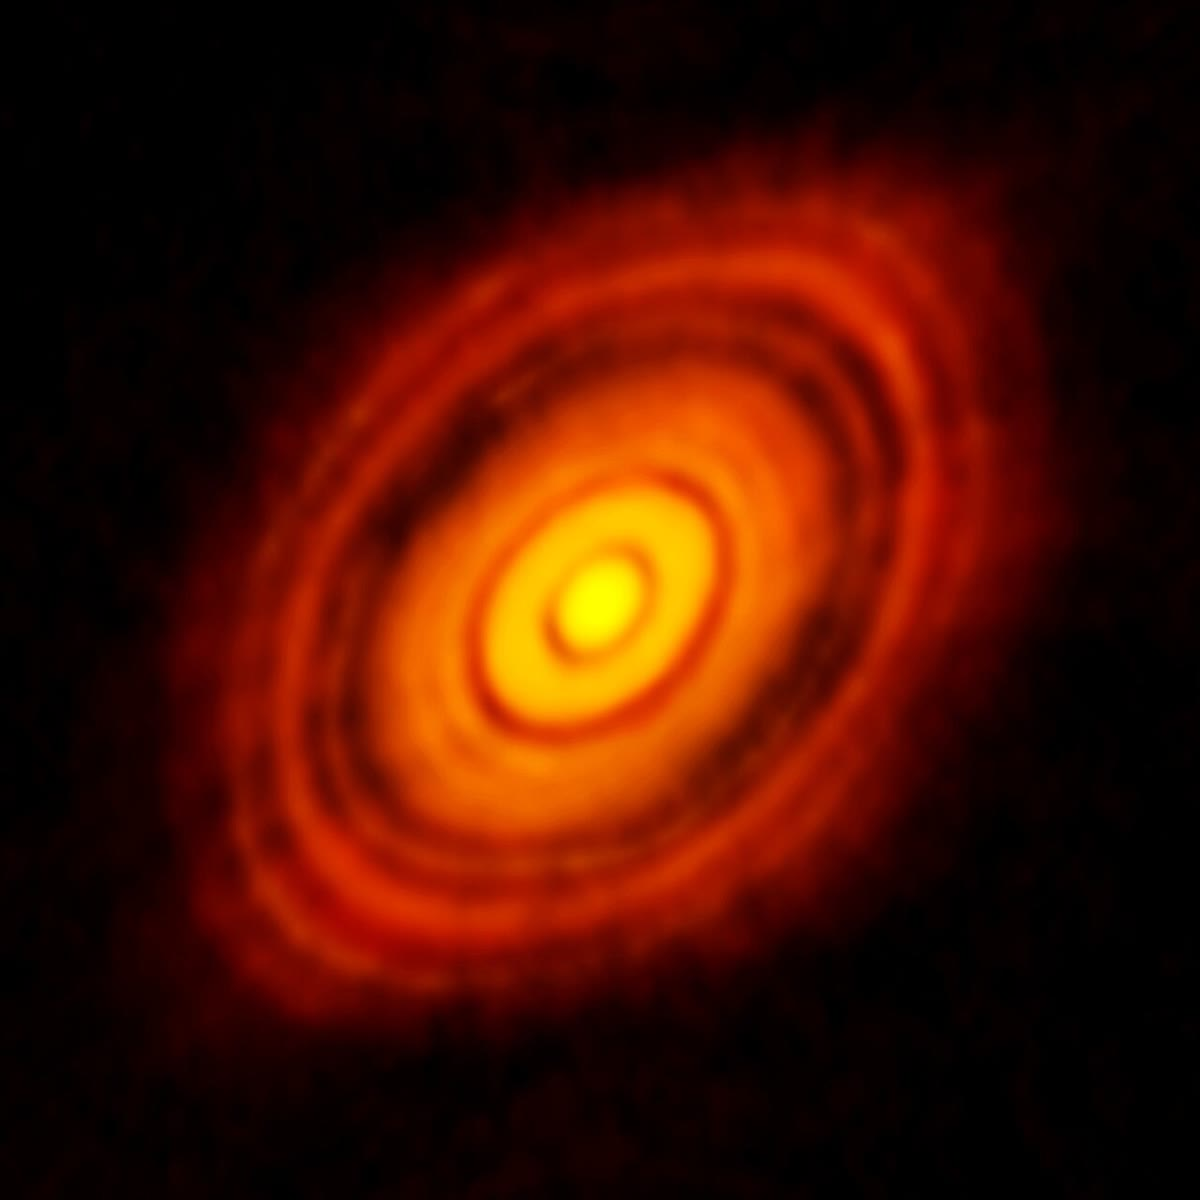
\includegraphics[width=\linewidth]{images/book4/b2-hl-tau-alma.jpg}
\end{minipage}\hfill
\begin{minipage}[c]{0.52\linewidth}
{\small De schijf van de jonge ster HL Tauri, op \qty{140}{pc} in de Stier, vastgelegd
door de ALMA-interferometer op een golflengte van ongeveer één millimeter, waar koud
stof straalt. De schijf, met een straal van ongeveer \qty{120}{au} en onder een hoek van
\ang{47} gezien, vertoont heldere en donkere ringen van enkele astronomische eenheden breed; het
stelsel is hoogstens een of twee miljoen jaar oud, en de ringen worden gelezen als de
eerste tekenen van planeten die hun baan vrijmaken. ALMA (ESO/NAOJ/NRAO), CC BY 4.0.}
\end{minipage}
% ledger: alma:hltau
\end{omfigure}

De schijf wordt door de ster verwarmd. Een korrel op afstand $r$ absorbeert sterlicht
over zijn doorsnede en straalt uit over zijn hele oppervlak.

\begin{proposition}[Temperatuur van een korrel in sterlicht]
\label{prop:b2:ism-star-formation:grain}
Een kleine korrel die zich als een zwart lichaam gedraagt, op afstand $r$ van een ster met
lichtkracht $L$ en slechts aan één kant belicht, komt op de temperatuur
\[
  T = \left(\frac{L}{16\pi\sigma r^2}\right)^{1/4},
\]
die afneemt als $r^{-1/2}$.
\end{proposition}

\begin{proof}
Een bolvormige korrel met straal $a$ onderschept het vermogen $\pi a^2\,L/(4\pi r^2)$
en straalt bij de temperatuur $T$ over zijn oppervlak $4\pi a^2\sigma T^4$ uit.
In evenwicht zijn beide gelijk: $T^4 = L/(16\pi\sigma r^2)$; $a$ valt weg.
\end{proof}

Op \qty{1}{au} van een ster als de Zon heeft de korrel \qty{278}{K}; op
\qty{5.2}{au}, waar Jupiter draait, \qty{122}{K}. Waterijs condenseert waar
de korrels kouder zijn dan ongeveer \qty{180}{K} (de condensatietemperaturen zijn
die van \cref{ch:b2:planet-formation-meteorites}), dat wil zeggen voorbij ongeveer
\qty{2.4}{au}: het eerste teken van de grens, de sneeuwlijn, die
rotsachtige van ijzige planeten scheidt. Een echte schijf is ondoorzichtig, en zijn middenvlak is afgeschermd van direct sterlicht; de
propositie geeft de juiste grootteorde en de juiste helling voor de
oppervlaktelagen die de ster ziet.
% ledger: lodders:tc-table

Schijven blijven niet bestaan. Een infraroodexces, de gloed van warm stof boven wat de ster
alleen zou uitzenden, verraadt of een ster nog een schijf heeft. Door de sterren
met zo'n exces te tellen in sterrenhopen van verschillende leeftijd, vindt men de fractie van de sterren
die hun schijf behouden als functie van de tijd (figuur hieronder): de meeste sterren hebben er een
bij hun geboorte, de helft heeft hem rond drie miljoen jaar verloren, en bijna geen enkele
houdt er een langer dan zes. Gasreuzen, die hun gas uit de schijf moeten halen,
moeten binnen deze paar miljoen jaar ontstaan.
% ledger: haisch:disc-fractions, haisch:disc-lifetime

\begin{omfigure}
\begin{tikzpicture}
\begin{axis}[omrecord, width=0.8\linewidth, height=5.6cm, xmin=0, xmax=8.5, ymin=0, ymax=1.05,
  xlabel={leeftijd van de sterrenhoop (Myr)}, ylabel={fractie sterren met een schijf},
  tick label style={font=\scriptsize}, label style={font=\small}, clip=false]
\addplot[thick, black!55, densely dashed] table[x=age, y=frac] {figdata/out/bachelor-2-jeans-discfit.dat};
\addplot[only marks, mark=*, mark size=1.8pt, blue!70!black,
  error bars/.cd, y dir=both, y explicit]
  table[x=age, y=frac, y error=err, restrict x to domain=0:10] {figdata/out/bachelor-2-jeans-discs.dat};
\node[font=\scriptsize, anchor=north west] at (axis cs:0.05,0.74) {NGC 2024};
\node[font=\scriptsize, anchor=south west] at (axis cs:1.55,0.86) {Trapezium};
\node[font=\scriptsize, anchor=south west] at (axis cs:2.35,0.71) {IC 348};
\node[font=\scriptsize, anchor=south west] at (axis cs:3.3,0.56) {NGC 2264};
\node[font=\scriptsize, anchor=south west] at (axis cs:5.1,0.15) {NGC 2362};
\node[font=\scriptsize, anchor=north east] at (axis cs:8.4,0.98) {(NGC 1960, \qty{30}{Myr}: $0.03$)};
\end{axis}
\end{tikzpicture}

\par\smallskip{\small Fractie van de sterren van jonge sterrenhopen die het infraroodexces
van een schijf vertonen, tegen de leeftijd van de sterrenhoop (met zijn fout), naar Haisch, Lada
en Lada (2001). De gestreepte lijn is de kleinste-kwadratenrechte door de vijf
jongste sterrenhopen: ze bereikt $0.5$ bij \qty{3.0}{Myr} en nul bij \qty{6.1}{Myr}
(\cref{exo:b2:ism-star-formation:12}).}
\end{omfigure}

\begin{inthelab}[Met radiogolven door het stof heen kijken]
\begin{minipage}[t]{0.55\linewidth}\vspace{0pt}
Koud gas en stof zijn onzichtbaar voor optische telescopen, maar stralen op
millimetergolflengten, waar de atmosfeer alleen boven hooggelegen, droge plaatsen doorzichtig is. Een
radioschotel ter grootte van een huis onderscheidt op zulke golflengten weinig, dus
combineren astronomen er vele: in een interferometer meet elk paar antennes, gescheiden
door een basislijn, één component van het helderheidspatroon van de hemel, en
een computer stelt het beeld samen uit de honderden paren die een dertigtal antennes vormen. Het oplossend vermogen is dat van
één enkele telescoop zo breed als de langste basislijn: met antennes verspreid over
\qty{15}{km} werd de schijf van HL Tauri afgebeeld met details van enkele astronomische eenheden op
\qty{140}{pc}. Operators verplaatsen de antennes met transportvoertuigen tussen opstellingen,
en de correlator combineert hun signalen in reële tijd.
\end{minipage}\hfill
\begin{minipage}[t]{0.42\linewidth}\vspace{0pt}
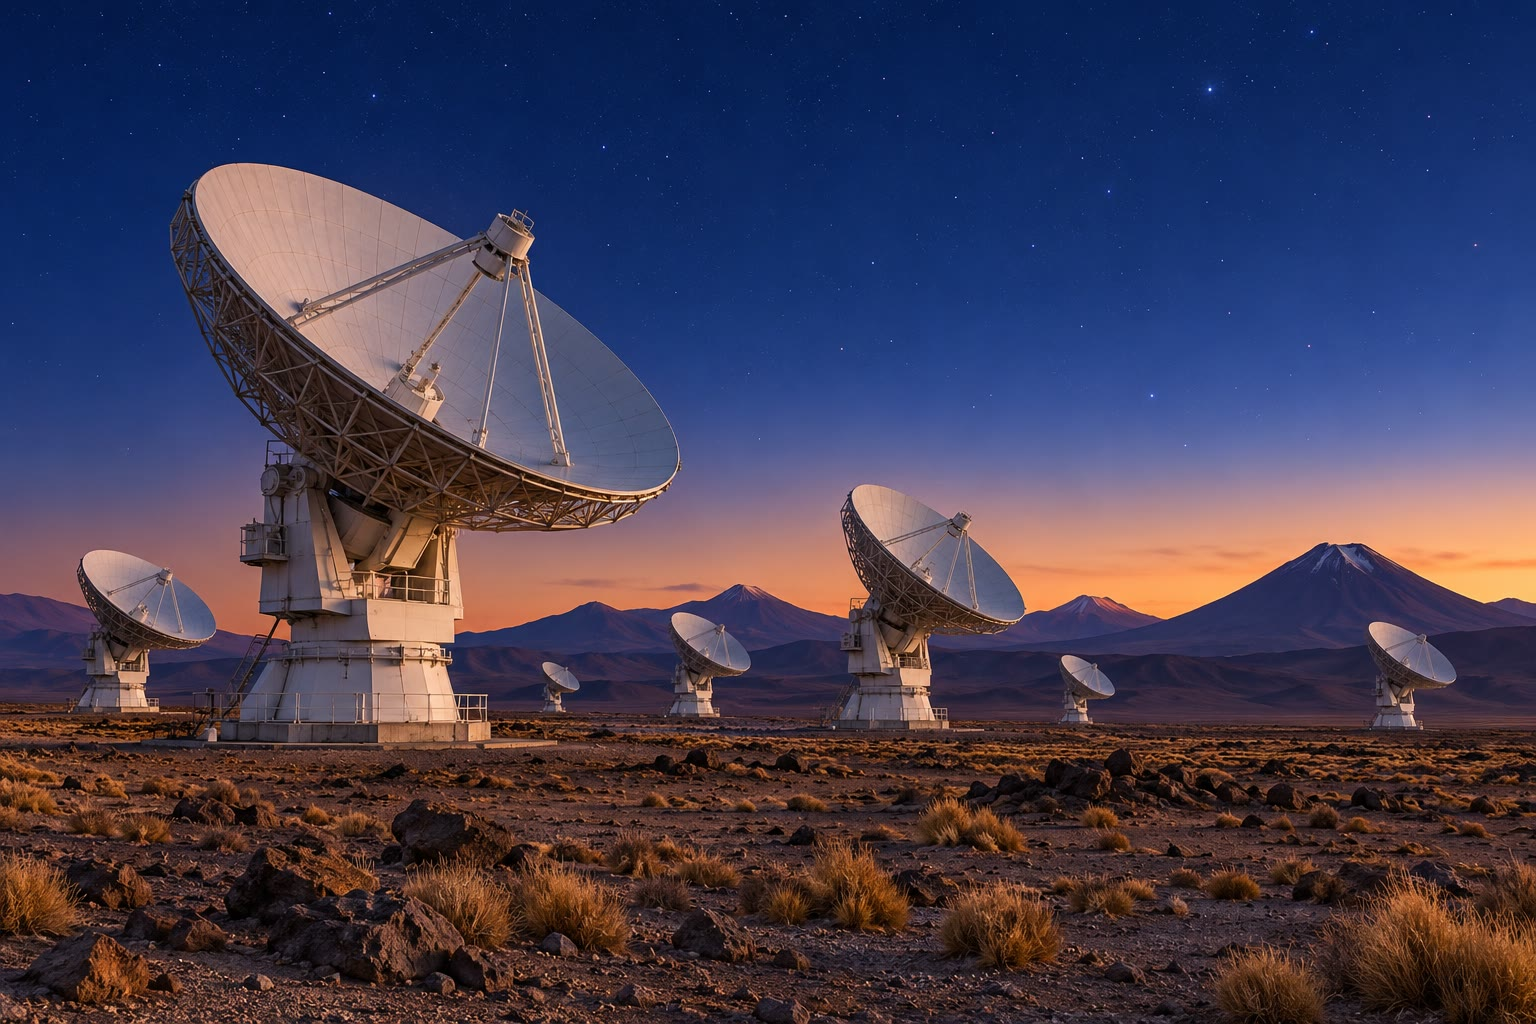
\includegraphics[width=\linewidth]{images/book4/ai/b2-radio-array.jpg}

{\scriptsize Een rij radioantennes op een hoge woestijnvlakte bij schemering
(door AI gegenereerde illustratie).}
\end{minipage}
% ledger: alma:hltau, alma:baselines
\end{inthelab}

\section{Oefeningen}

\begin{exercise}[$\star$]\label{exo:b2:ism-star-formation:1}
De gemiddelde interstellaire dichtheid nabij de Zon is \qty{2.7e-24}{g.cm^{-3}}. Neem
voor de massa van een waterstofatoom \qty{1.67e-24}{g} en bereken het aantal
waterstofatomen per kubieke centimeter. Vergelijk met het aantal moleculen per kubieke
centimeter in lucht bij \qty{101325}{Pa} en \qty{288}{K} ($n = P/k_{\mathrm B}T$).
% ledger: ferriere:mean-density, const:kB
\end{exercise}

\begin{exercise}[$\star$]\label{exo:b2:ism-star-formation:2}
Bereken met de waarde $M_J = 5.46$ zonsmassa's bij \qty{10}{K} en $10^4$ deeltjes
per kubieke centimeter, en met de schaling van $M_J$ met de dichtheid, de \omterm{def:b2:ism-star-formation:jeans}{Jeans-massa}
bij \qty{10}{K} en $10^2$ deeltjes per kubieke centimeter. Hoeveel \omterm{def:b2:ism-star-formation:jeans}{Jeans-massa}'s
bevat de wolk in de Stier, \num{24000} zonsmassa's?
% ledger: goldsmith:taurus-mass
\end{exercise}

\begin{exercise}[$\star$]\label{exo:b2:ism-star-formation:3}
Bereken de isotherme geluidssnelheid $c_s = (k_{\mathrm B}T/\mu m_u)^{1/2}$ van
moleculair gas ($\mu = 2.33$, $m_u = \qty{1.661e-27}{kg}$) bij \qty{10}{K} en bij
\qty{100}{K}. Hoe lang doet een geluidsgolf erover om bij \qty{10}{K} een kern met straal
\qty{0.1}{pc} te doorkruisen, in miljoenen jaren?
% ledger: kauffmann:mu, nist:u, iau:parsec
\end{exercise}

\begin{exercise}[$\star$]\label{exo:b2:ism-star-formation:4}
Bereken de \omterm{def:b2:ism-star-formation:free-fall}{vrijevaltijd} van een \omterm{def:b2:ism-star-formation:molecular-cloud}{dichte kern} van $10^5$ deeltjes per kubieke
centimeter en van een donkere wolk van $10^2$ ($\mu = 2.33$). Welke stort
sneller in, en met welke factor?
\end{exercise}

\begin{exercise}[$\star\star$]\label{exo:b2:ism-star-formation:5}
Toon aan dat $M_J$ kan worden geschreven als $M_J = 5^{3/2}\,(3/4\pi)^{1/2}\,c_s^3\,G^{-3/2}\rho^{-1/2}$.
Met welke factor moet bij vaste temperatuur de dichtheid van een kern stijgen om
zijn \omterm{def:b2:ism-star-formation:jeans}{Jeans-massa} te halveren? Met welke factor verandert bij vaste dichtheid de \omterm{def:b2:ism-star-formation:jeans}{Jeans-massa} als
de kern opwarmt van \qty{10}{K} tot \qty{20}{K}?
\end{exercise}

\begin{exercise}[$\star\star$]\label{exo:b2:ism-star-formation:6}
Een jonge ster heeft de massa van de Zon, twee keer haar straal en twee keer haar lichtkracht
($M_\odot = \qty{1.989e30}{kg}$, $R_\odot = \qty{6.96e8}{m}$,
$L_\odot = \qty{3.83e26}{W}$). Bereken haar Kelvin--Helmholtz-tijd in miljoenen
jaren, en vergelijk met de levensduur van schijven.
% ledger: sun:mass, sun:R, sun:L
\end{exercise}

\begin{exercise}[$\star\star$]\label{exo:b2:ism-star-formation:7}
Bereken het accretietempo $c_s^3/G$ van een \omterm{def:b2:ism-star-formation:protostar}{protoster} in een kern van \qty{10}{K}, in
zonsmassa's per jaar, en de tijd die ze nodig heeft om één zonsmassa te verzamelen. Dezelfde
vragen voor een kern van \qty{20}{K}.
\end{exercise}

\begin{exercise}[$\star\star$]\label{exo:b2:ism-star-formation:8}
Bereken met \cref{prop:b2:ism-star-formation:grain} en $L_\odot = \qty{3.83e26}{W}$
de afstand tot de Zon, in astronomische eenheden, waarop een korrel
\qty{1300}{K} bereikt, dicht bij de temperatuur waarbij de gewone silicaten
condenseren (\cref{ch:b2:planet-formation-meteorites}), en
de temperatuur van een korrel op de afstand van Jupiter, \qty{5.2}{au}.
% ledger: sun:L, const:sigma, const:au
\end{exercise}

\begin{exercise}[$\star\star$]\label{exo:b2:ism-star-formation:9}
Het gas van de schijf van HL Tauri draait rond een ster van ongeveer \num{1.3}
zonsmassa. Bereken de Kepleriaanse snelheid en de omlooptijd op \qty{100}{au}.
Als het stelsel een miljoen jaar oud is, hoeveel omlopen heeft het gas op
\qty{100}{au} dan gemaakt sinds de ster ontstond?
% ledger: alma:hltau
\end{exercise}

\begin{exercise}[$\star\star\star$]\label{exo:b2:ism-star-formation:10}
Bepaal de gravitatie-energie van een bol met straal $R$ waarin de dichtheid
afneemt als $\rho(r) = \rho_0 R/r$, en vergelijk ze met die van een homogene bol met
dezelfde massa en straal. Maakt het concentreren van de massa naar het centrum
de wolk gemakkelijker of moeilijker te dragen door haar thermische energie?
\end{exercise}

\begin{exercise}[$\star\star\star$]\label{exo:b2:ism-star-formation:11}
Een kern met straal \qty{0.1}{pc} roteert als een star lichaam met de hoeksnelheid
$\Omega = \qty{1e-14}{rad.s^{-1}}$. Bereken zijn rotatieperiode, het specifieke
impulsmoment $j = \Omega R^2$ van gas aan zijn evenaar, en de centrifugale
straal van dat gas rond een ster van één zonsmassa, in astronomische eenheden.
Waarom komt gas uit het binnenste van de kern dichter bij de ster terecht?
\end{exercise}

\begin{exercise}[$\star\star\star$]\label{exo:b2:ism-star-formation:12}
De schijffracties van de vijf jongste sterrenhopen van de figuur in de laatste
paragraaf zijn $0.85$, $0.80$, $0.65$, $0.52$ en $0.12$ bij 0.3, 1.5, 2.3, 3.2 en
\qty{5.0}{Myr}. Pas met de hand een kleinste-kwadratenrechte $f = a - bt$ aan
(bereken de gemiddelden, dan $\sum(t - \bar t)(f - \bar f)$ en
$\sum(t - \bar t)^2$). Bij welke leeftijd bereikt ze een half, en nul? Waarom is een
rechte lijn voorbij die leeftijd een slecht model?
% ledger: haisch:disc-fractions
\end{exercise}

\section{Probleem: Een kern in de Aldra-wolk}

\begin{problem}[{Weekendprobleem --- de massa en de stabiliteit van een dichte kern, afgelezen van een
stofkaart, de geboorte van zijn protoster en de grootte van zijn schijf}]
\label{pb:b2:ism-star-formation:1}
% values: calc/ch01.py
% ledger: kauffmann:mu, nist:u, iau:parsec, const:G, const:kB, sun:mass, sun:R, sun:L, const:au, const:sigma, bt07:cores, alma:hltau
De Aldra-wolk is een verzonnen donkere wolk. Een millimeterkaart van haar stof
toont een ronde kern met straal \qty{0.08}{pc} en een gemiddelde kolomdichtheid van
$N(\ce{H2}) = \num{1.5e22}$ waterstofmoleculen per vierkante centimeter. Een
ammoniaklijn geeft de gastemperatuur, \qty{10}{K}, en een snelheidsgradiënt
van \qty{0.4}{km.s^{-1}} per parsec over de kern, gelezen als rotatie van een star
lichaam. Gebruik $G = \qty{6.674e-11}{m^3.kg^{-1}.s^{-2}}$,
$k_{\mathrm B} = \qty{1.381e-23}{J.K^{-1}}$, $m_u = \qty{1.661e-27}{kg}$,
\qty{1}{pc} $= \qty{3.086e16}{m}$, \qty{1}{au} $= \qty{1.496e11}{m}$, een jaar van
\qty{3.156e7}{s}, $M_\odot = \qty{1.989e30}{kg}$, $R_\odot = \qty{6.96e8}{m}$,
$L_\odot = \qty{3.83e26}{W}$, $\sigma = \qty{5.67e-8}{W.m^{-2}.K^{-4}}$; de
massa per waterstofmolecuul, helium inbegrepen, is $2.8\,m_u$, en de gemiddelde massa
per deeltje $2.33\,m_u$.

\medskip
\noindent\textbf{Deel I --- Massa en dichtheid.}
\begin{enumerate}
  \item Reken de straal van de kern om naar meter.
  \item Bereken de massa per vierkante meter van de kolom, $2.8\,m_u N$.
  \item Leid daaruit de massa van de kern af, in kilogram en in zonsmassa's.
  \item Bereken zijn volume en zijn gemiddelde dichtheid.
  \item Bereken het aantal deeltjes per kubieke centimeter.
  \item Is dit een \omterm{def:b2:ism-star-formation:molecular-cloud}{dichte kern} in de zin van de tabel van de tweede paragraaf?
\end{enumerate}

\noindent\textbf{Deel II --- Stabiliteit.}
\begin{enumerate}[resume]
  \item Bereken de \omterm{def:b2:ism-star-formation:jeans}{Jeans-massa} van het gas van de kern, in zonsmassa's.
  \item Hoeveel \omterm{def:b2:ism-star-formation:jeans}{Jeans-massa}'s bevat de kern? Is hij stabiel?
  \item Bereken de \omterm{def:b2:ism-star-formation:jeans}{Jeans-lengte} en vergelijk die met de straal van de kern.
  \item Hoe groot zou de \omterm{def:b2:ism-star-formation:jeans}{Jeans-massa} zijn als het gas \qty{20}{K} had? Zou de
        kern dan nog ineenstorten?
  \item Bereken de \omterm{def:b2:ism-star-formation:free-fall}{vrijevaltijd} van de kern, in duizenden jaren.
  \item Vergelijk die met de tijd die een geluidsgolf nodig heeft om de kern te doorkruisen. Welk
        proces is sneller, en wat betekent dat?
\end{enumerate}

\noindent\textbf{Deel III --- De protoster.}
\begin{enumerate}[resume]
  \item Bereken de geluidssnelheid in de kern.
  \item Bereken het accretietempo $c_s^3/G$, in zonsmassa's per jaar.
  \item Bereken de tijd die nodig is om bij dit tempo één zonsmassa te verzamelen.
  \item Als een derde van de kern in sterren eindigt, hoeveel sterren van één zonsmassa
        kan hij dan vormen?
  \item Wanneer de omhulling verdwenen is, heeft de ster één zonsmassa, drie
        zonsstralen en vier zonslichtkrachten. Bereken haar Kelvin--Helmholtz-tijd.
  \item Is die langer of korter dan de accretietijd? Wat voor ster is het
        dan?
\end{enumerate}

\noindent\textbf{Deel IV --- De schijf.}
\begin{enumerate}[resume]
  \item Reken de snelheidsgradiënt om naar een hoeksnelheid $\Omega$, in
        \unit{rad.s^{-1}}.
  \item Bereken het specifieke impulsmoment $j = \Omega R^2$ van gas aan de
        evenaar van de kern.
  \item Bereken zijn centrifugale straal rond een ster van één zonsmassa, in
        astronomische eenheden.
  \item Bereken de temperatuur van een korrel op \qty{1}{au} en op \qty{30}{au}
        van een ster met één zonslichtkracht.
  \item Waar ligt de sneeuwlijn van deze schijf, als waterijs onder
        \qty{180}{K} overleeft?
  \item Geef de tijd die nodig is om de ster van vraag 15 op te bouwen, het kerngetal
        van dit probleem, in duizenden jaren, en vergelijk die met de
        \omterm{def:b2:ism-star-formation:free-fall}{vrijevaltijd} van vraag 11.
\end{enumerate}
\end{problem}
